\chapter{Development of the chosen solutions}

El nom d’aquest apartat s'ha de triar en funció del treball que es porti a terme. Aquest apartat pot constar de diversos apartats i subapartats, depenent del criteri de l‘autor o autora i de les consideracions de la tesi que es desenvolupa.

\section{Graphic interface}

About user friendly graphic interface..................................

\section{Settings page}

About parameters that can be set on this page, an why we need them.

\section{Signal Path}
	
How is adquired data from soundcard and how I move this thata inside the program

\section{Acoustics analysis}

The acoustic analysis is devoloped with python librari LIBROSA\cite{librosa}

\subsection{Spectrogram (FT)}

How implemented the spectogram

\subsection{RTA}

Usually, any form of analysis that is performed in real time can be considered \textbf{RTA} (\textit{Real-Time Analysis}). This includes a wide range of operations such as spectrum monitoring, transfer function measurements, phase and coherence analysis, and more—all happening as the signal flows. However, in my experience, in common usage, when someone refers to "RTA", they are often specifically referring to the classic 31-band graphical spectrum display. Also, the data collected on this page is especially important because it will be used to set the correction parameters. For all of that, this page has been named \textbf{RTA}.

Also, there is another conflict. When someone defines the 31 bands and their bandwidth, it is common to use the definition provided in \textbf{IEC 61260}. However, this standard does not mathematically respect the logarithmic spacing between bands. The 31 bands are defined as 1/3 of an octave per band.

\begin{table}[H]
\centering
\caption{Center frequencies for true 1/3 octave bands and IEC 61260 bands} 

	\scalebox{0.53}{
		\begin{tabular}{|c|c|c|c|c|c|c|c|c|c|c|c|}
			\hline
			1/3 octave & 20 & 25.18 & 31.7 & 39.91 & 50.24 & 63.25 & 79.62 & 100.24 & 126.19 & 158.87 & \\ \hline
			IEC 61260 & 20 & 25 & 31.5 & 40 & 50 & 63 & 80 & 100 & 125 & 160 & \\ \hline
			 & & & & & & & & & & & \\ \hline
			1/3 octave & 200 & 251.79 & 316.98 & 399.05 & 502.38 & 632.46 & 796.21 & 1002.37 & 1261.91 & 1588.66 & \\ \hline
			IEC 61260 & 200 & 250 & 315 & 400 & 500 & 630 & 800 & 1000 & 1250 & 1600 & \\ \hline
			 & & & & & & & & & & & \\ \hline
			1/3 octave & 2000 & 2517.85 & 3169.79 & 3990.52 & 5023.77 & 6324.56 & 7962.14 & 10023.74 & 12619.15 & 15886.56 & 20000 \\ \hline
			IEC 61260 & 2000 & 2500 & 3150 & 4000 & 5000 & 6300 & 8000 & 10000 & 12500 & 16000 & 20000 \\ \hline
				
		\end{tabular}
	}
\end{table}

\begin{minted}[label=\texttt{ipython}]{python3}
	"""
	In order to obtain the true 1/3 octave values, the following line of code was used with IPython3.
	The results were rounded to the second decimal place.
	"""
	
	import numpy as np
	print(np.round(np.logspace(np.log10(20), np.log10(20000), 31), 2)) 
	
\end{minted}

On the other hand, this standard is widely used in many professional devices and software. One important example is the DBX 231s graphic equalizer, which is commonly used in analog processing chains.

\begin{figure}[H]
	\centering
	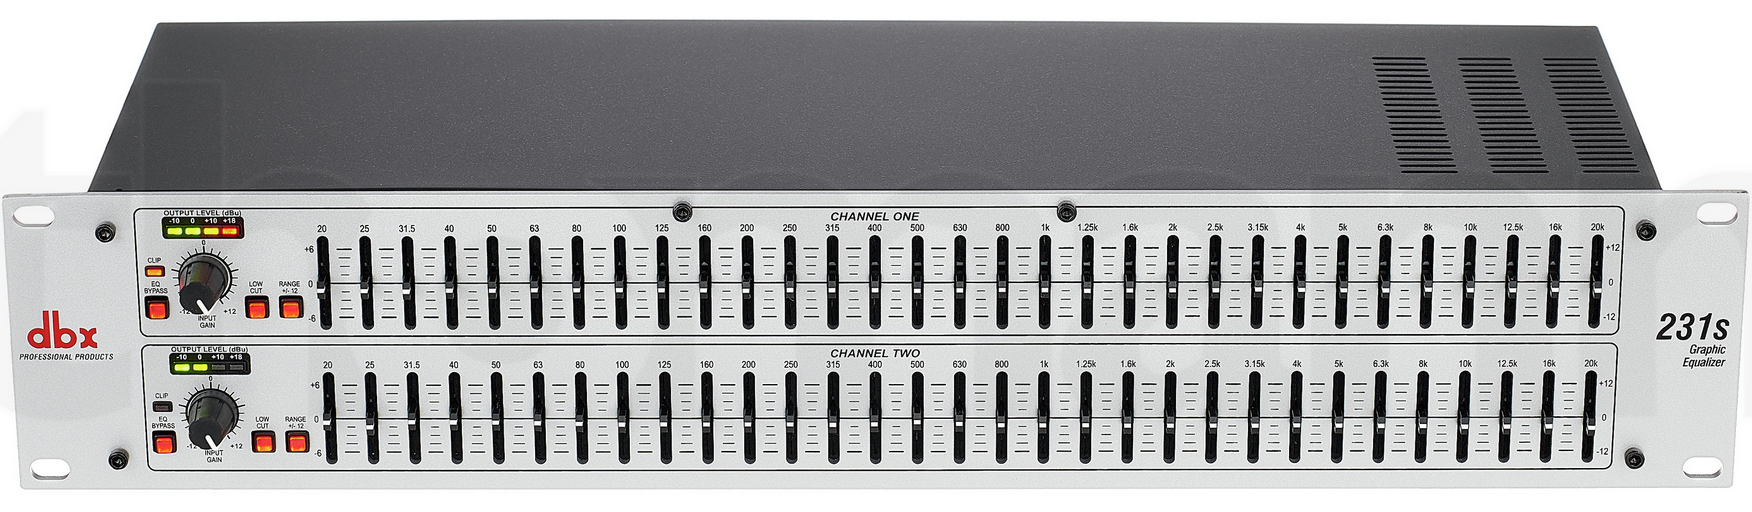
\includegraphics[width=1
	\linewidth]{Figures/DBX_231s.png}
	\caption{Image of the front panel of the DBX 231s \cite{DBX_31s}, where we can observe that the center frequency bands are the same as those defined in IEC 61260.}
	\label{fig:DBX_31s}
\end{figure}

In order to achieve the greatest possible compatibility and coherence with industry standards, I prefer to use the IEC 61260 standard.


The signal path on this page is very similar to the one used on the "FT" page. We have a buffer with two blocks of input data ("In from external device" and "In from system").

First, we copy the buffer data to the "delay buffer", where, if needed, the data will be adjusted to make it coincide with the applied delay. If necessary, the adjustment will use data from previous blocks stored in the same "delay buffer".

I created this buffer with the capacity to store 1 second of data, which can be used to apply a maximum delay of (1 - "Block Size in seconds") seconds.

Once the data in the "delay buffer" is adjusted, we can start applying algorithms to perform the analysis.

The algorithm is based on the calculation of RMS (\textit{root mean square}) to obtain the energy for each frequency band, which is divided using filters for each band.


\begin{figure}[H]
	\begin{center}
		\vspace{-2mm}
		\tikzsetnextfilename{RTA_page_schem}
		\begin{tikzpicture}[node distance=30mm,on grid,auto, scale=1, bend angle=45]
			
			every node/.style={font=\small};
			
			\node (q_init) [draw, rectangle, minimum size=1cm,] {Input Buffer};
			\node (null_init) [right=of q_init] {};
			\node (q_delay) [draw, rectangle, minimum size=1cm, right=of null_init] {Delay Buffer};
			\node (q_ext) [draw, rectangle, minimum size=1cm, above right=of q_delay, xshift=2cm] {Filtering and RMS Calculation of External Input};
			\node (q_in_sys) [draw, rectangle, minimum size=1cm, below right=of q_delay, xshift=2cm] {Filtering and RMS Calculation of Input from System};
			\node (q_diff) [draw, rectangle, minimum size=1cm, right=of q_delay, xshift=4cm] {Difference calculation};	
			
			\draw[blue, very thick, ->] (q_init) edge node {2 channels} (q_delay);
			\draw[blue, dotted, very thick, ->] (q_delay) edge[bend right=10] node {1 channel} (q_ext);
			\draw[blue, dotted, very thick, ->] (q_delay) edge[bend right=10] node {1 channel} (q_in_sys);
			\draw[green, very thick, ->] (q_ext) edge[bend right=10] node {Analysis Data} (q_diff);
			\draw[green, very thick, ->] (q_in_sys) edge[bend right=10] node {Analysis Data} (q_diff);
			
		\end{tikzpicture}
		\vspace{-2mm}
	\end{center}
	\caption{Diagram of the architecture of the RTA page}
\end{figure}


In this case, I'm not using any kind of windowing. As a starting point, I'm using 4th-order IIR (\textit{infinite impulse response}) Butterworth band-pass filters for each band. All these filters are created using the \texttt{scipy.signal} library \cite{scipy_signal}, which returns SOS (\textit{Second-Order Section}) parameters.

\begin{figure}[H]
	\centering
	\caption{Second-Order Sections for IIR filters with their parameters}
	\[
	H(z) = \frac{b_0 + b_1 z^{-1} + b_2 z^{-2}}{1 + a_1 z^{-1} + a_2 z^{-2}}
	\]
\end{figure}

When the program applies each filter to the signal block, it also calculates the RMS and converts it to a logarithmic scale, which will be plotted on the graph and used to calculate the difference graph.

\begin{figure}[H]
	\centering
	\caption{Root Mean Square to calculate energy from filtered signal}
	\[
	RMS = \sqrt{ \frac{1}{N} \sum_{n=0}^{N-1} x^2[n] }
	\]
\end{figure}

At the end, there is: a pause button, which blocks the update function and can be used to pause the graphics; a save button, to store the current values of the difference graph for later use in the correction window; and a time averaging section that works exactly the same as the averaging section from the FT page, except that it does not include frequency averaging (since it doesn't make sense to apply frequency averaging between bands).

\begin{figure}[H]
	\centering
	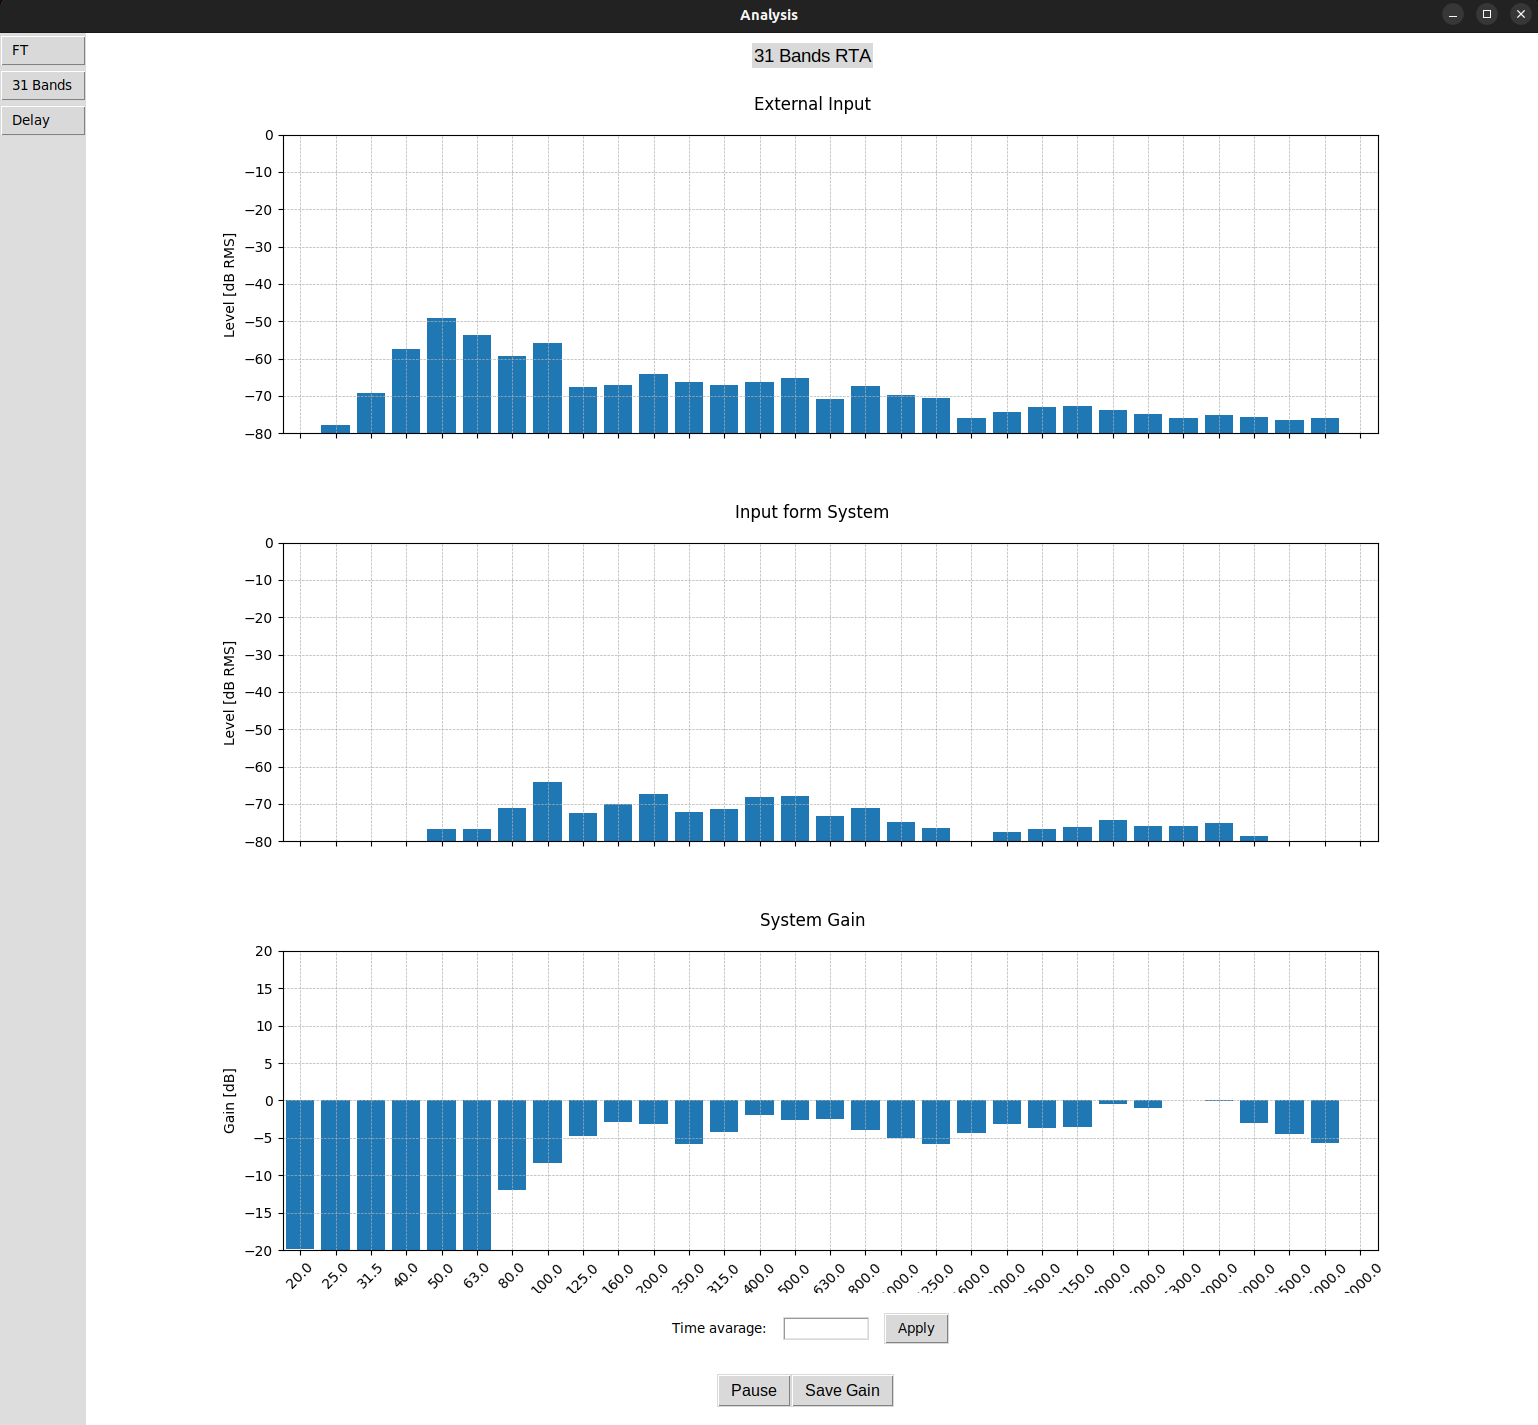
\includegraphics[width=1
	\linewidth]{Figures/RTA_page.png}
	\caption{Analysis window - RTA page.}
	\label{fig:DBX_31s}
\end{figure}


\subsection{Delay}

Explain delay page

\section{Acoustic correction}

Acoustic correction = DSP, allways have to be somethuing on the output buffer, by default, zeros.

\subsection{Bypass}

How Bypass works, and why it works bad.

\subsection{31 Bars}

Implementation of correction

\section{Integration of monitoring mechanism}

Home page and information that it appears / start, stop streams buttons...

\section{Others}

More problems that I didn't expect, losing time solving them or at least trying to. No more time to implement additional functionalities...